% SPDX-License-Identifier: CC-BY-SA-4.0
%
% Copyright (C) 2026 embedded brains GmbH & Co. KG
\documentclass[tikz,border=4pt]{standalone}
\usepackage[T1]{fontenc}
\usepackage[scaled]{helvet}
\renewcommand{\familydefault}{\sfdefault}
\usetikzlibrary{arrows.meta,backgrounds,positioning,calc}
\definecolor{ebblue}{HTML}{1F4E79}
\definecolor{boxfill}{HTML}{EAF1F8}
\definecolor{codefill}{HTML}{FFF4E0}
\definecolor{codeline}{HTML}{9C6500}
\definecolor{groupfill}{HTML}{F5F5F5}
\definecolor{flow}{HTML}{404040}
\begin{document}
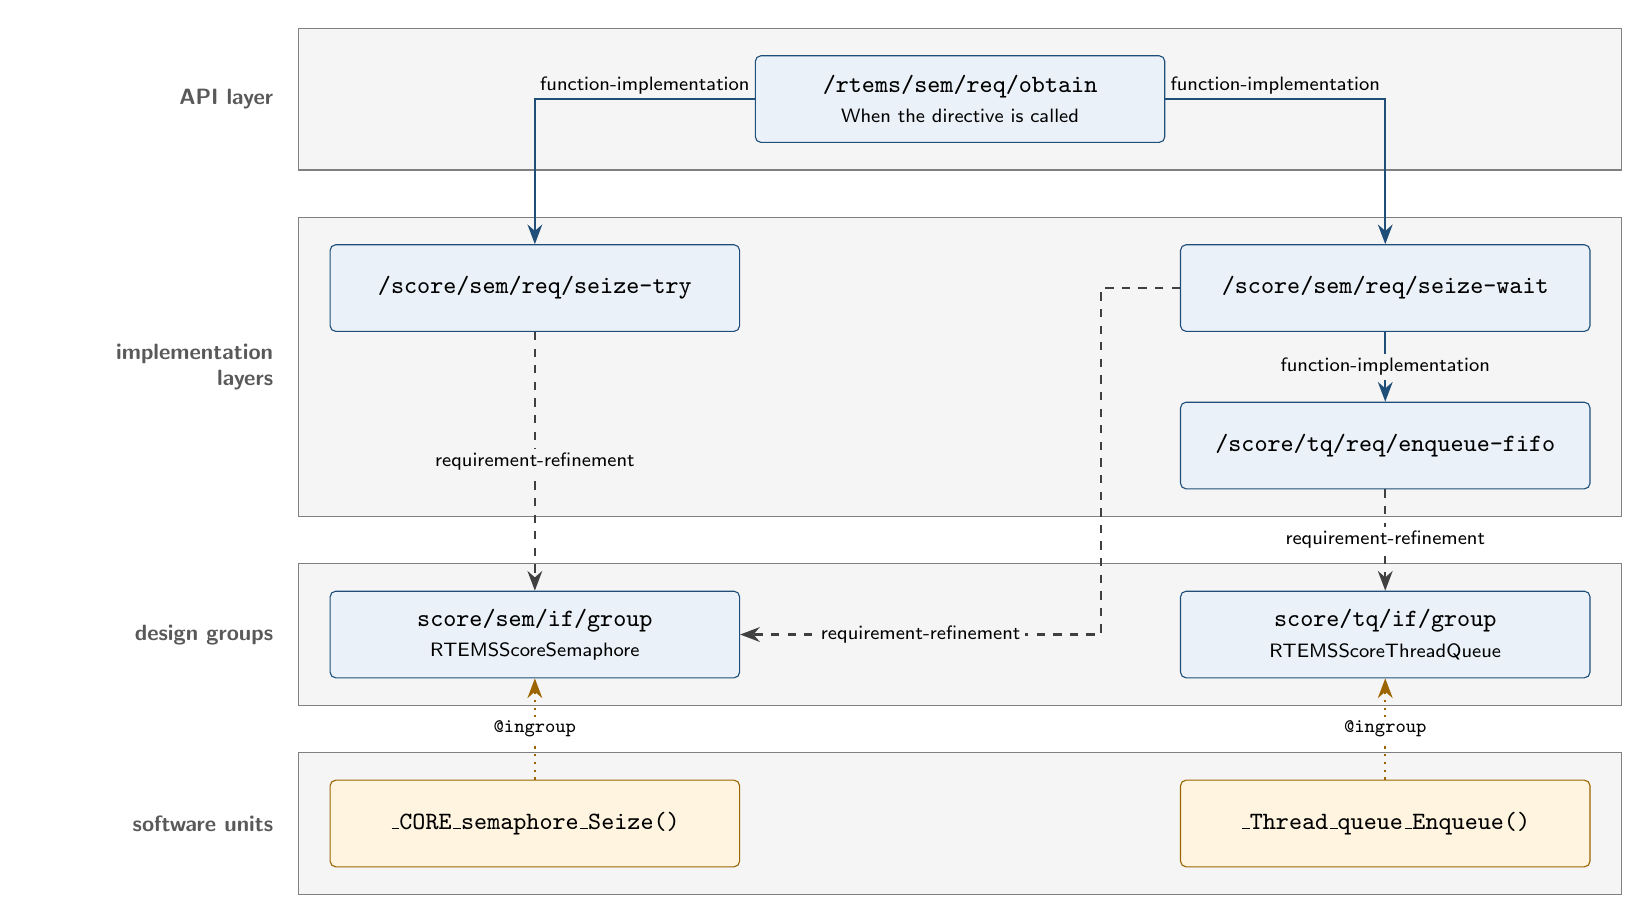
\begin{tikzpicture}[
    font=\small,
    req/.style={draw=ebblue, fill=boxfill, rounded corners=2pt,
      minimum width=52mm, minimum height=11mm, align=center},
    unit/.style={draw=codeline, fill=codefill, rounded corners=2pt,
      minimum width=52mm, minimum height=11mm, align=center},
    lanelabel/.style={font=\footnotesize\bfseries, text=gray!70!black,
      align=right, anchor=east, text width=30mm},
    impl/.style={-{Stealth[length=2.5mm]}, thick, draw=ebblue},
    refine/.style={-{Stealth[length=2.5mm]}, thick, dashed, draw=flow},
    ingroup/.style={-{Stealth[length=2.5mm]}, thick, dotted, draw=codeline},
    lbl/.style={font=\scriptsize, fill=groupfill, inner sep=1.5pt}]

  \def\xa{1.4}\def\xb{6.8}\def\xc{12.2}
  \def\left{-1.6}\def\right{15.2}
  \foreach \y/\h/\name in {9.2/0.9/API layer, 5.8/1.9/implementation\\layers,
      2.4/0.9/design groups, 0/0.9/software units} {
    \fill[groupfill] (\left,\y-\h) rectangle (\right,\y+\h);
    \draw[gray] (\left,\y-\h) rectangle (\right,\y+\h);
    \node[lanelabel] at (\left-0.2,\y) {\name};
  }

  \node[req] (obtain) at (\xb,9.2)
    {\texttt{/rtems/sem/req/obtain}\\\scriptsize When the directive is called};
  \node[req] (wait) at (\xc,6.8) {\texttt{/score/sem/req/seize-wait}};
  \node[req] (try) at (\xa,6.8) {\texttt{/score/sem/req/seize-try}};
  \node[req] (fifo) at (\xc,4.8) {\texttt{/score/tq/req/enqueue-fifo}};
  \node[req] (semgroup) at (\xa,2.4)
    {\texttt{score/sem/if/group}\\\scriptsize RTEMSScoreSemaphore};
  \node[req] (tqgroup) at (\xc,2.4)
    {\texttt{score/tq/if/group}\\\scriptsize RTEMSScoreThreadQueue};
  \node[unit] (seize) at (\xa,0) {\texttt{\_CORE\_semaphore\_Seize()}};
  \node[unit] (enqueue) at (\xc,0) {\texttt{\_Thread\_queue\_Enqueue()}};

  \draw[impl] (obtain.west) -| node[lbl, pos=0.25, above, fill=none] {function-implementation}
    (try.north);
  \draw[impl] (obtain.east) -| node[lbl, pos=0.25, above, fill=none]
    {function-implementation} (wait.north);
  \draw[impl] (wait) -- node[lbl] {function-implementation} (fifo);
  \draw[refine] (try) -- node[lbl] {requirement-refinement} (semgroup);
  \draw[refine] (fifo) -- node[lbl, fill=white] {requirement-refinement} (tqgroup);
  \draw[refine] (wait.west) -- ++(-1.0,0) coordinate (bend)
    |- node[lbl, pos=0.75] {requirement-refinement} (semgroup.east);
  \draw[ingroup] (seize) -- node[lbl, fill=white] {\texttt{@ingroup}} (semgroup);
  \draw[ingroup] (enqueue) -- node[lbl, fill=white] {\texttt{@ingroup}} (tqgroup);
\end{tikzpicture}
\end{document}
